% =========================================================================
% results.tex
% =========================================================================

\section{Results}
\label{sec:results}

% -----------------------------------------------------------------
\subsection{Main Comparison}
\label{sec:results:main}

Table~\ref{tab:main} presents the primary benchmark results. Because the outlier-split variants require a different token-window evaluation protocol, their perplexity metrics are not directly comparable to the WikiText-2 full-context baselines. To ensure clarity and avoid misleading comparison, the results are separated into two blocks: Sub-Table 2a for the full-context baselines and Sub-Table 2b for the outlier channel splitting configurations.

\begin{table}[ht]
\vspace{-4pt}
\centering
\caption{Main comparison of quantization schemes on GPT-2 Medium
($\dhead = 64$). We report WikiText-2 strided perplexity (1{,}024-token sliding window) for full-context evaluations, and short-context average perplexity (50-token window) for outlier-split configurations. Because the outlier-split variants require a different token-window evaluation protocol, their perplexity metrics are not directly comparable to the WikiText-2 full-context baselines.}
\label{tab:main}

\medskip
\textbf{Sub-Table 2a: Full-Context Quantization Baselines} \\
\vspace{2pt}
\footnotesize
\begin{tabular}{@{}>{\raggedright\arraybackslash}p{4.5cm}cccccc@{}}
\toprule
\textbf{Scheme} & \textbf{Total} & \textbf{Comp.} & \textbf{WT-2} & \textbf{Hella-} & \textbf{NIAH} & \textbf{NN} \\
 & \textbf{Bits} & \textbf{Ratio} & \textbf{Str. PPL} & \textbf{Swag} & \textbf{@512m} & \textbf{R@1} \\
\midrule
Baseline FP16   & 16.00 & 1.00$\times$ & 19.03 & 40.0 & 100.0 & --- \\
TurboQuant (3-bit base + 1-bit QJL) & 4.00 & 4.00$\times$ & 89.34 & 37.0 & --- & 14.0 \\
TurboQuant (4-bit base + 1-bit QJL) & 5.00 & 3.20$\times$ & 24.71 & 38.0 & 100.0 & 38.8 \\
WHT + Asymmetric (3-bit base + 1-bit QJL) & 4.00 & 4.00$\times$ & 76.93 & 42.0 & --- & 46.4 \\
WHT + Asymmetric (4-bit base + 1-bit QJL) & 5.00 & 3.20$\times$ & 23.95 & 40.0 & 100.0 & 67.4 \\
MC-TurboQuant (4-bit base + 1-bit QJL)    & 5.00 & 3.20$\times$ & 23.95 & 40.0 & 100.0 & 67.4 \\
\bottomrule
\end{tabular}

\vspace{4pt}
\textbf{Sub-Table 2b: Outlier Channel Splitting Results} \\
\vspace{2pt}
\footnotesize
\begin{tabular}{@{}lcccc@{}}
\toprule
\textbf{Scheme} & \textbf{Bits} & \textbf{Comp. Ratio} & \textbf{Short-Ctx PPL} & \textbf{NN R@1} \\
\midrule
Outlier (2.5-bit) & 3.44 & 4.65$\times$ & 4.68 & 29.8 \\
Outlier (3.5-bit) & 4.44 & 3.60$\times$ & 5.56 & 48.2 \\
\bottomrule
\end{tabular}
\vspace{-4pt}
\end{table}

The primary empirical result demonstrates the benefit of disabling the QJL residual correction: at four-bit,
WHT + Asymmetric achieves 67.4\% Recall@1 versus 38.8\% for flat
TurboQuant, a relative improvement of 73.7\%, by simply bypassing
the residual calculation that introduces harmful variance at
$\dhead = 64$.
WikiText-2 strided perplexity also improves modestly (23.95 versus
24.71).
HellaSwag zero-shot accuracy remains within two percentage points of
the FP16 baseline across all schemes.

MC-TurboQuant matches the WHT + Asymmetric scheme on all metrics while
adding the segment-level memory caching infrastructure, demonstrating
that GRM integration incurs no measurable quality penalty.

% -----------------------------------------------------------------
\subsection{Nearest-Neighbor Retrieval}
\label{sec:results:nn}

We evaluate nearest-neighbor retrieval capabilities across a spectrum of bit allocations.

\begin{table}[ht]
\vspace{-4pt}
\centering
\caption{Nearest-neighbor retrieval performance at $\dhead = 64$ across
quantization schemes and bit rates.
Recall@$k$ measures the fraction of true top-$k$ neighbors recovered
from the quantized representations.
Mean rank is the average rank of the true nearest neighbor in the
quantized ranking.
All values from \texttt{results/nn\_search.json}.}
\label{tab:nn}
\footnotesize
\begin{tabular}{@{}llcccc@{}}
\toprule
\textbf{Scheme} & \textbf{Bits} & \textbf{R@1 (\%)} & \textbf{R@10 (\%)}
  & \textbf{Mean Rank} & \textbf{Comp.} \\
\midrule
Flat TurboQuant & 2 &  2.8 &  9.8 & 511.4 & 5.33$\times$ \\
Flat TurboQuant & 3 & 14.0 & 48.0 &  54.9 & 4.00$\times$ \\
Flat TurboQuant & 4 & 38.8 & 87.6 &   5.8 & 3.20$\times$ \\
\midrule
WHT + Asymmetric & 2 & 22.4 & 63.6 &  18.5 & 6.40$\times$ \\
WHT + Asymmetric & 3 & 46.4 & 94.4 &   3.3 & 4.57$\times$ \\
WHT + Asymmetric & 4 & 67.4 & 99.8 &   1.7 & 3.56$\times$ \\
\midrule
Outlier Split & 2.5 & 29.8 & 73.8 &  14.0 & 5.82$\times$ \\
Outlier Split & 3.5 & 48.2 & 94.8 &   3.3 & 4.27$\times$ \\
\bottomrule
\end{tabular}
% Source: results/nn_search.json — all values verbatim
%   flat_turboquant/2: R@1=2.8, R@10=9.8, mean_rank=511.4, CR=5.33
%   flat_turboquant/3: R@1=14.0, R@10=48.0, mean_rank=54.9, CR=4.00
%   flat_turboquant/4: R@1=38.8, R@10=87.6, mean_rank=5.8, CR=3.20
%   wht_asym/2: R@1=22.4, R@10=63.6, mean_rank=18.5, CR=6.40
%   wht_asym/3: R@1=46.4, R@10=94.4, mean_rank=3.3, CR=4.57
%   wht_asym/4: R@1=67.4, R@10=99.8, mean_rank=1.7, CR=3.56
%   outlier_split/2.5: R@1=29.8, R@10=73.8, mean_rank=14.0, CR=5.82
%   outlier_split/3.5: R@1=48.2, R@10=94.8, mean_rank=3.3, CR=4.27
\vspace{-4pt}
\end{table}

The WHT + Asymmetric scheme dominates flat TurboQuant at every bit rate.
At two-bit, the gap is largest in relative terms: 22.4\% versus 2.8\%
Recall@1, an eight-fold improvement.
The outlier split scheme occupies an intermediate position, offering
competitive recall at fractional bit rates that are not directly
available to the flat schemes.

% -----------------------------------------------------------------
\subsection{Distortion-Rate Analysis}
\label{sec:results:distortion}

Figure~\ref{fig:distortion} plots the empirical MSE distortion against
the Shannon rate-distortion lower bound
$D^*(R) = \sigma^2 \cdot 2^{-2R}$
for unit-variance Gaussian sources~\cite{shannon1959coding}.
I evaluate five quantization schemes (Uniform, Lloyd-Max without
rotation, TurboQuant MSE with QR rotation, WHT + Lloyd-Max, and
Outlier-split WHT) from one to six bits.

\begin{figure}[ht]
\vspace{-4pt}
\vspace{-6pt}
\centering
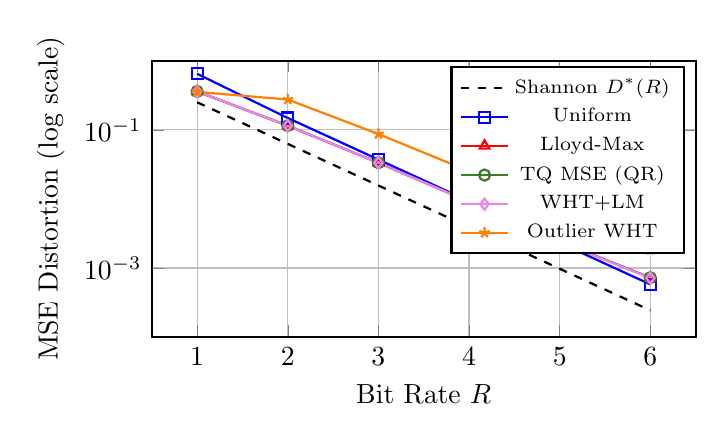
\begin{tikzpicture}
\begin{axis}[
    width=0.70\columnwidth,
    height=0.42\columnwidth,
    xlabel={Bit Rate $R$},
    ylabel={MSE Distortion (log scale)},
    ymode=log,
    xmin=0.5, xmax=6.5,
    ymin=1e-4, ymax=1,
    grid=major,
    legend style={font=\scriptsize, at={(0.98,0.98)}, anchor=north east},
    cycle list name=color list,
    mark size=2pt,
    line width=0.8pt
]

% Shannon bound
\addplot[black, dashed, thick, no markers, domain=1:6, samples=6]
    {0.25^x};
\addlegendentry{Shannon $D^*(R)$}

% Uniform
\addplot[mark=square, blue] coordinates {
    (1,0.6453) (2,0.1481) (3,0.0371) (4,0.00928) (5,0.00232) (6,0.000580)
};
\addlegendentry{Uniform}

% Lloyd-Max (No Rotation)
\addplot[mark=triangle, red] coordinates {
    (1,0.3580) (2,0.1144) (3,0.0334) (4,0.00915) (5,0.00241) (6,0.000725)
};
\addlegendentry{Lloyd-Max}

% TurboQuant MSE (Flat QR)
\addplot[mark=o, OliveGreen] coordinates {
    (1,0.3586) (2,0.1147) (3,0.0334) (4,0.00914) (5,0.00241) (6,0.000725)
};
\addlegendentry{TQ MSE (QR)}

% WHT + Lloyd-Max
\addplot[mark=diamond, Violet] coordinates {
    (1,0.3585) (2,0.1146) (3,0.0334) (4,0.00912) (5,0.00240) (6,0.000718)
};
\addlegendentry{WHT+LM}

% Outlier-split WHT
\addplot[mark=star, orange] coordinates {
    (1,0.3531) (2,0.2741) (3,0.0869) (4,0.0252) (5,0.00691) (6,0.00183)
};
\addlegendentry{Outlier WHT}

\end{axis}
\end{tikzpicture}
\vspace{-6pt}
\caption{Rate-distortion curves at $\dhead = 64$.
All rotation-based schemes (TQ~MSE, WHT+LM) track the Shannon bound
closely, remaining within 1.83--2.46$\times$ across two to five bits.
The outlier-split scheme trades higher distortion for better
channel-level precision allocation.
Data from \texttt{results/distortion\_rate.json}.}
\label{fig:distortion}
% Source: results/distortion_rate.json — all coordinate values
\vspace{-4pt}
\end{figure}

The rotation-based schemes (TurboQuant MSE and WHT + Lloyd-Max) are
nearly indistinguishable and track the Shannon bound closely.
At four-bit, the WHT scheme achieves MSE = 0.00912, which is
$2.34{\times}$ the Shannon bound of $0.00391$.
Across two to five bits, the ratio for WHT ranges from 1.83 to 2.46,
well within the theoretical $\leq 4{\times}$ bound for scalar quantizers
established in~\cite{zandieh2025turboquant}.
% Source: results/distortion_bounds.json → ratio_wht:
%   2-bit: 1.833, 3-bit: 2.137, 4-bit: 2.336, 5-bit: 2.457

The outlier-split scheme exhibits higher MSE because it allocates
precision non-uniformly: outlier channels receive more bits at the
expense of normal channels, optimizing for channel-level fidelity rather
than global MSE.

% -----------------------------------------------------------------
\subsection{MQAR: Limitations of Zero-Shot Evaluation}
\label{sec:results:mqar}

MQAR accuracy is 0\% across all aggregation schemes (Baseline, RM, GRM,
SSC) when evaluated zero-shot on GPT-2 Medium, with only sporadic
non-zero values (10\% for Baseline and GRM at sequence length 128 with
8~key-value pairs).
% Source: results/mc_variants.json — all values 0.0 except
%   baseline/128/8 = 10.0 and grm/128/8 = 10.0

This reflects a limitation of the base model, not of the implementation:
GPT-2 Medium has not been instruction-tuned to parse the synthetic
key-value query format that MQAR requires (\eg,
``red $\rightarrow$ one, blue $\rightarrow$ two $\ldots$ query:
red $\rightarrow$'').
The original Memory Caching paper~\cite{behrouz2026mc} trains models
from scratch specifically on MQAR data (Section~5.5 of that paper).
By contrast, NIAH recall reaches 100\% in this setting because its
prompts are natural-language question-answer pairs that the base model
was already pretrained to handle.
I report this null result for completeness and transparency rather than
omitting it.
The full MQAR table is provided in Appendix~\ref{app:mqar}.
